
\documentclass[letterpaper,hide notes,xcolor={table,svgnames},pdftex,10pt]{beamer}
\def\showexamples{t}


%\usepackage[svgnames]{xcolor}

%% Demo talk
%\documentclass[letterpaper,notes=show]{beamer}

\usecolortheme{crane}
\setbeamertemplate{navigation symbols}{}

\usetheme{MyPittsburgh}
%\usetheme{Frankfurt}

%\usepackage{tipa}

\usepackage{hyperref}
\usepackage{graphicx,xspace}
\usepackage[normalem]{ulem}
\usepackage{multicol}
\usepackage{amsmath,amssymb,amsthm,graphicx,xspace}
\newcommand\SF[1]{$\bigstar$\footnote{SF: #1}}

\usepackage[default]{sourcesanspro}
\usepackage[T1]{fontenc}
\usepackage[scaled]{beramono}
\usepackage{tikzpagenodes}

\newcounter{tmpnumSlide}
\newcounter{tmpnumNote}


% old question code
%\newcommand\question[1]{{$\bigstar$ \small \onlySlide{2}{#1}}}
% \newcommand\nquestion[1]{\ifdefined \presentationonly \textcircled{?} \fi \note{\par{\Large \textbf{?}} #1}}
% \newcommand\nanswer[1]{\note{\par{\Large \textbf{A}} #1}}


 \newcommand\mnote[1]{%
   \addtocounter{tmpnumSlide}{1}
   \ifdefined\showcues {~\tiny\fbox{\arabic{tmpnumSlide}}}\fi
   \note{\setlength{\parskip}{1ex}\addtocounter{tmpnumNote}{1}\textbf{\Large \arabic{tmpnumNote}:} {#1\par}}}

\newcommand\mmnote[1]{\note{\setlength{\parskip}{1ex}#1\par}}

%\newcommand\mnote[2][]{\ifdefined\handoutwithnotes {~\tiny\fbox{#1}}\fi
% \note{\setlength{\parskip}{1ex}\textbf{\Large #1:} #2\par}}

%\newcommand\mnote[2][]{{\tiny\fbox{#1}} \note{\setlength{\parskip}{1ex}\textbf{\Large #1:} #2\par}}

\newcommand\mquestion[2]{{~\color{red}\fbox{?}}\note{\setlength{\parskip}{1ex}\par{\Large \textbf{?}} #1} \note{\setlength{\parskip}{1ex}\par{\Large \textbf{A}} #2\par}\ifdefined \presentationonly \pause \fi}

\newcommand\blackboard[1]{%
\ifdefined   \showblackboard
  {#1}
  \else {\begin{center} \fbox{\colorbox{blue!30}{%
         \begin{minipage}{.95\linewidth}%
           \hspace{\stretch{1}} Some space intentionally left blank; done at the blackboard.%
         \end{minipage}}}\end{center}}%
         \fi%
}



%\newcommand\q{\tikz \node[thick,color=black,shape=circle]{?};}
%\newcommand\q{\ifdefined \presentationonly \textcircled{?} \fi}

\usepackage{listings}
\lstset{basicstyle=\footnotesize\ttfamily,
	breaklines=true,
	aboveskip=15pt,
  	belowskip=15pt,
	frame=lines,
	numbers=left, basicstyle=\scriptsize, numberstyle=\tiny, stepnumber=0, numbersep=2pt
}

\usepackage{siunitx}
\newcommand\sius[1]{\num[group-separator = {,}]{#1}\si{\micro\second}}
\newcommand\sims[1]{\num[group-separator = {,}]{#1}\si{\milli\second}}
\newcommand\sins[1]{\num[group-separator = {,}]{#1}\si{\nano\second}}
\sisetup{group-separator = {,}, group-digits = true}

%% -------------------- tikz --------------------
\usepackage{tikz}
\usetikzlibrary{positioning}
\usetikzlibrary{arrows,backgrounds,automata,decorations.shapes,decorations.pathmorphing,decorations.markings,decorations.text,decorations.pathreplacing}

\tikzstyle{place}=[circle,draw=blue!50,fill=blue!20,thick, inner sep=0pt,minimum size=6mm]
\tikzstyle{transition}=[rectangle,draw=black!50,fill=black!20,thick, inner sep=0pt,minimum size=4mm]

\tikzstyle{block}=[rectangle,draw=black, thick, inner sep=5pt]
\tikzstyle{bullet}=[circle,draw=black, fill=black, thin, inner sep=2pt]

\tikzstyle{pre}=[<-,shorten <=1pt,>=stealth',semithick]
\tikzstyle{post}=[->,shorten >=1pt,>=stealth',semithick]
\tikzstyle{bi}=[<->,shorten >=1pt,shorten <=1pt, >=stealth',semithick]

\tikzstyle{mut}=[-,>=stealth',semithick]

\tikzstyle{treereset}=[dashed,->, shorten >=1pt,>=stealth',thin]

\usepackage{ifmtarg}
\usepackage{xifthen}
\makeatletter
% new counter to now which frame it is within the sequence
\newcounter{multiframecounter}
% initialize buffer for previously used frame title
\gdef\lastframetitle{\textit{undefined}}
% new environment for a multi-frame
\newenvironment{multiframe}[1][]{%
\ifthenelse{\isempty{#1}}{%
% if no frame title was set via optional parameter,
% only increase sequence counter by 1
\addtocounter{multiframecounter}{1}%
}{%
% new frame title has been provided, thus
% reset sequence counter to 1 and buffer frame title for later use
\setcounter{multiframecounter}{1}%
\gdef\lastframetitle{#1}%
}%
% start conventional frame environment and
% automatically set frame title followed by sequence counter
\begin{frame}%
\frametitle{\lastframetitle~{\normalfont(\arabic{multiframecounter})}}%
}{%
\end{frame}%
}
\makeatother

\makeatletter
\newdimen\tu@tmpa%
\newdimen\ydiffl%
\newdimen\xdiffl%
\newcommand\ydiff[2]{%
    \coordinate (tmpnamea) at (#1);%
    \coordinate (tmpnameb) at (#2);%
    \pgfextracty{\tu@tmpa}{\pgfpointanchor{tmpnamea}{center}}%
    \pgfextracty{\ydiffl}{\pgfpointanchor{tmpnameb}{center}}%
    \advance\ydiffl by -\tu@tmpa%
}
\newcommand\xdiff[2]{%
    \coordinate (tmpnamea) at (#1);%
    \coordinate (tmpnameb) at (#2);%
    \pgfextractx{\tu@tmpa}{\pgfpointanchor{tmpnamea}{center}}%
    \pgfextractx{\xdiffl}{\pgfpointanchor{tmpnameb}{center}}%
    \advance\xdiffl by -\tu@tmpa%
}
\makeatother
\newcommand{\copyrightbox}[3][r]{%
\begin{tikzpicture}%
\node[inner sep=0pt,minimum size=2em](ciimage){#2};
\usefont{OT1}{phv}{n}{n}\fontsize{4}{4}\selectfont
\ydiff{ciimage.south}{ciimage.north}
\xdiff{ciimage.west}{ciimage.east}
\ifthenelse{\equal{#1}{r}}{%
\node[inner sep=0pt,right=1ex of ciimage.south east,anchor=north west,rotate=90]%
{\raggedleft\color{black!50}\parbox{\the\ydiffl}{\raggedright{}#3}};%
}{%
\ifthenelse{\equal{#1}{l}}{%
\node[inner sep=0pt,right=1ex of ciimage.south west,anchor=south west,rotate=90]%
{\raggedleft\color{black!50}\parbox{\the\ydiffl}{\raggedright{}#3}};%
}{%
\node[inner sep=0pt,below=1ex of ciimage.south west,anchor=north west]%
{\raggedleft\color{black!50}\parbox{\the\xdiffl}{\raggedright{}#3}};%
}
}
\end{tikzpicture}
}


%% --------------------

%\usepackage[excludeor]{everyhook}
%\PushPreHook{par}{\setbox0=\lastbox\llap{MUH}}\box0}

%\vspace*{\stretch{1}

%\setbox0=\lastbox \llap{\textbullet\enskip}\box0}

\setlength{\parskip}{\fill}

\newcommand\noskips{\setlength{\parskip}{1ex}}
\newcommand\doskips{\setlength{\parskip}{\fill}}

\newcommand\xx{\par\vspace*{\stretch{1}}\par}
\newcommand\xxs{\par\vspace*{2ex}\par}
\newcommand\tuple[1]{\langle #1 \rangle}
\newcommand\code[1]{{\sf \footnotesize #1}}
\newcommand\ex[1]{\uline{Example:} \ifdefined \presentationonly \pause \fi
  \ifdefined\showexamples#1\xspace\else{\uline{\hspace*{2cm}}}\fi}

\newcommand\ceil[1]{\lceil #1 \rceil}


\AtBeginSection[]
{
   \begin{frame}
       \frametitle{Outline}
       \tableofcontents[currentsection]
   \end{frame}
}



\pgfdeclarelayer{edgelayer}
\pgfdeclarelayer{nodelayer}
\pgfsetlayers{edgelayer,nodelayer,main}

\tikzstyle{none}=[inner sep=0pt]
\tikzstyle{rn}=[circle,fill=Red,draw=Black,line width=0.8 pt]
\tikzstyle{gn}=[circle,fill=Lime,draw=Black,line width=0.8 pt]
\tikzstyle{yn}=[circle,fill=Yellow,draw=Black,line width=0.8 pt]
\tikzstyle{empty}=[circle,fill=White,draw=Black]
\tikzstyle{bw} = [rectangle, draw, fill=blue!20, 
    text width=4em, text centered, rounded corners, minimum height=2em]
    
    \newcommand{\CcNote}[1]{% longname
	This work is licensed under the \textit{Creative Commons #1 3.0 License}.%
}
\newcommand{\CcImageBy}[1]{%
	\includegraphics[scale=#1]{creative_commons/cc_by_30.pdf}%
}
\newcommand{\CcImageSa}[1]{%
	\includegraphics[scale=#1]{creative_commons/cc_sa_30.pdf}%
}
\newcommand{\CcImageNc}[1]{%
	\includegraphics[scale=#1]{creative_commons/cc_nc_30.pdf}%
}
\newcommand{\CcGroupBySa}[2]{% zoom, gap
	\CcImageBy{#1}\hspace*{#2}\CcImageNc{#1}\hspace*{#2}\CcImageSa{#1}%
}
\newcommand{\CcLongnameByNcSa}{Attribution-NonCommercial-ShareAlike}

\newenvironment{changemargin}[1]{% 
  \begin{list}{}{% 
    \setlength{\topsep}{0pt}% 
    \setlength{\leftmargin}{#1}% 
    \setlength{\rightmargin}{1em}
    \setlength{\listparindent}{\parindent}% 
    \setlength{\itemindent}{\parindent}% 
    \setlength{\parsep}{\parskip}% 
  }% 
  \item[]}{\end{list}} 




\title{Lecture 20 --- Performance Case Studies}

\author{Patrick Lam \\ \small \texttt{patrick.lam@uwaterloo.ca}}
\institute{Department of Electrical and Computer Engineering \\
  University of Waterloo}
\date{\today}


\begin{document}

\begin{frame}
  \titlepage

\end{frame}


\part{Firefox}

\begin{frame}
\frametitle{Case Study: Firefox Quantum}

\begin{center}

\includegraphics[width=.6\textwidth]{images/L19-logo-quantum.png}
\end{center}

\end{frame}

\begin{frame}[fragile]
\frametitle{Some Firefox Perf Improvements, per Mike Conley}

\begin{minipage}{.5\textwidth}
\begin{itemize}
\item don't animate out-of-view elements
\item move db init off main thread
\item keep better profiling data
\item parallel painting for macOS
\item lazily instantiate Search Service
\end{itemize}
\end{minipage}\begin{minipage}{.5\textwidth}
\begin{itemize}
\item halve size of the blocklist
\item refactor to reduce main-thread IO
\item don't hold all frames of animated GIFs/APNGs in memory
\item eliminate unnecessary hash table
\item use more modern compiler
\end{itemize}
\end{minipage}

\begin{center}
\url{https://mikeconley.ca/blog/2018/02/14/firefox-performance-update-1/}
\end{center}

\end{frame}

\begin{frame}
\large
\frametitle{We've seen this before:}
\begin{itemize}
\item do less work (or do it sooner/later);
\item use threads (move work off main thread);
\item measure performance;
\end{itemize}
Which of the updates fall into which categories?
\end{frame}

\begin{frame}[fragile]
\frametitle{Some Firefox Perf Improvements, per Mike Conley}

\begin{minipage}{.5\textwidth}
\begin{itemize}
\item don't animate out-of-view elements
\item move db init off main thread
\item keep better profiling data
\item parallel painting for macOS
\item lazily instantiate Search Service
\end{itemize}
\end{minipage}\begin{minipage}{.5\textwidth}
\begin{itemize}
\item halve size of the blocklist
\item refactor to reduce main-thread IO
\item don't hold all frames of animated GIFs/APNGs in memory
\item eliminate unnecessary hash table
\item use more modern compiler
\end{itemize}
\end{minipage}

\begin{center}
\begin{minipage}{.6\textwidth}
\large How?
\begin{itemize}
\item do less work (or do it sooner/later);
\item use threads (move work off main thread);
\item measure performance;
\end{itemize}
\end{minipage}
\end{center}

\end{frame}

\begin{frame}
\frametitle{Tab Warming}
\begin{center}
\url{https://mikeconley.ca/blog/2018/01/11/making-tab-switching-faster-in-firefox-with-tab-warming/}.
\end{center}

\begin{minipage}[t]{.5\textwidth}
\vspace{0pt}
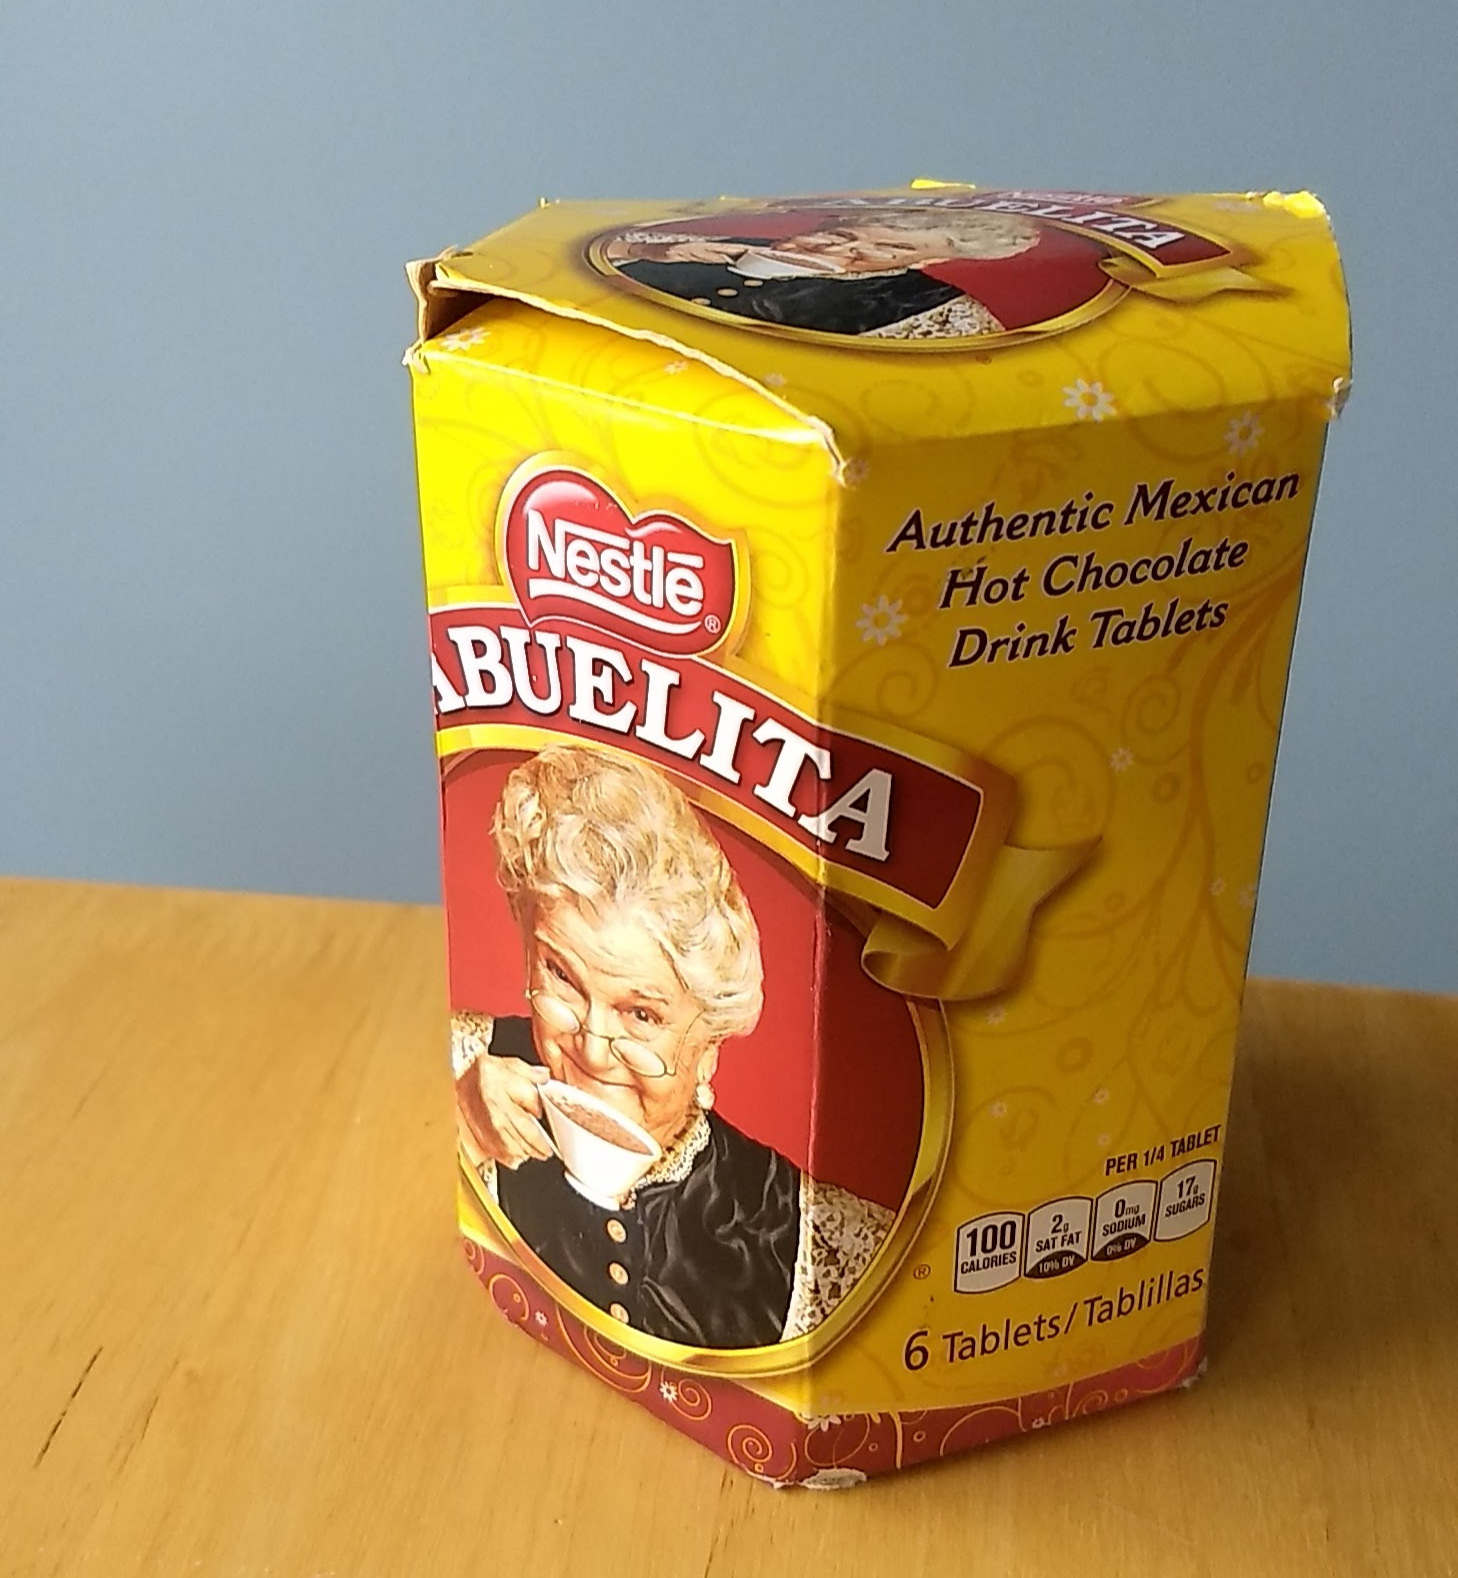
\includegraphics[width=.95\columnwidth]{images/L19-hot-chocolate.jpg}
\end{minipage}%
\begin{minipage}[t]{.5\textwidth}
\vspace{3em}
``Maybe this is my Canadian-ness showing, but I like to think of it almost like coming in from shoveling snow off of the driveway, and somebody inside has \emph{already made hot chocolate for you}, because they knew you’d probably be cold.'' --- Mike Conley
\end{minipage}

\end{frame}

\begin{frame}
\frametitle{How Can Tab Warming Work?}
\Large

Before: Firefox requests paint of newly-active tab,\\
and then waits for the result before switching.

Idea: reduce user-visible latency by predicting an imminent tab switch.

Q: How can we predict the future?

Q': How can we predict which tab will be switched to?

\end{frame}

\begin{frame}
\frametitle{Predicting the future}
\large

A: When the user has a mouse, then the mouse cursor will hover over the next tab.

\vspace*{1em}
\begin{quote}
Assuming a sufficiently long delay between hover and click, the tab switch should be perceived as instantaneous. If the delay was non-zero but still not long enough, we will have nonetheless shaved that time off in eventually presenting the tab to you.

And in the event that we were wrong, and you weren’t interested in seeing the tab, we eventually throw the uploaded layers away.
\end{quote}

Blog post does not report performance numbers.
\end{frame}

\begin{frame}
\begin{center}
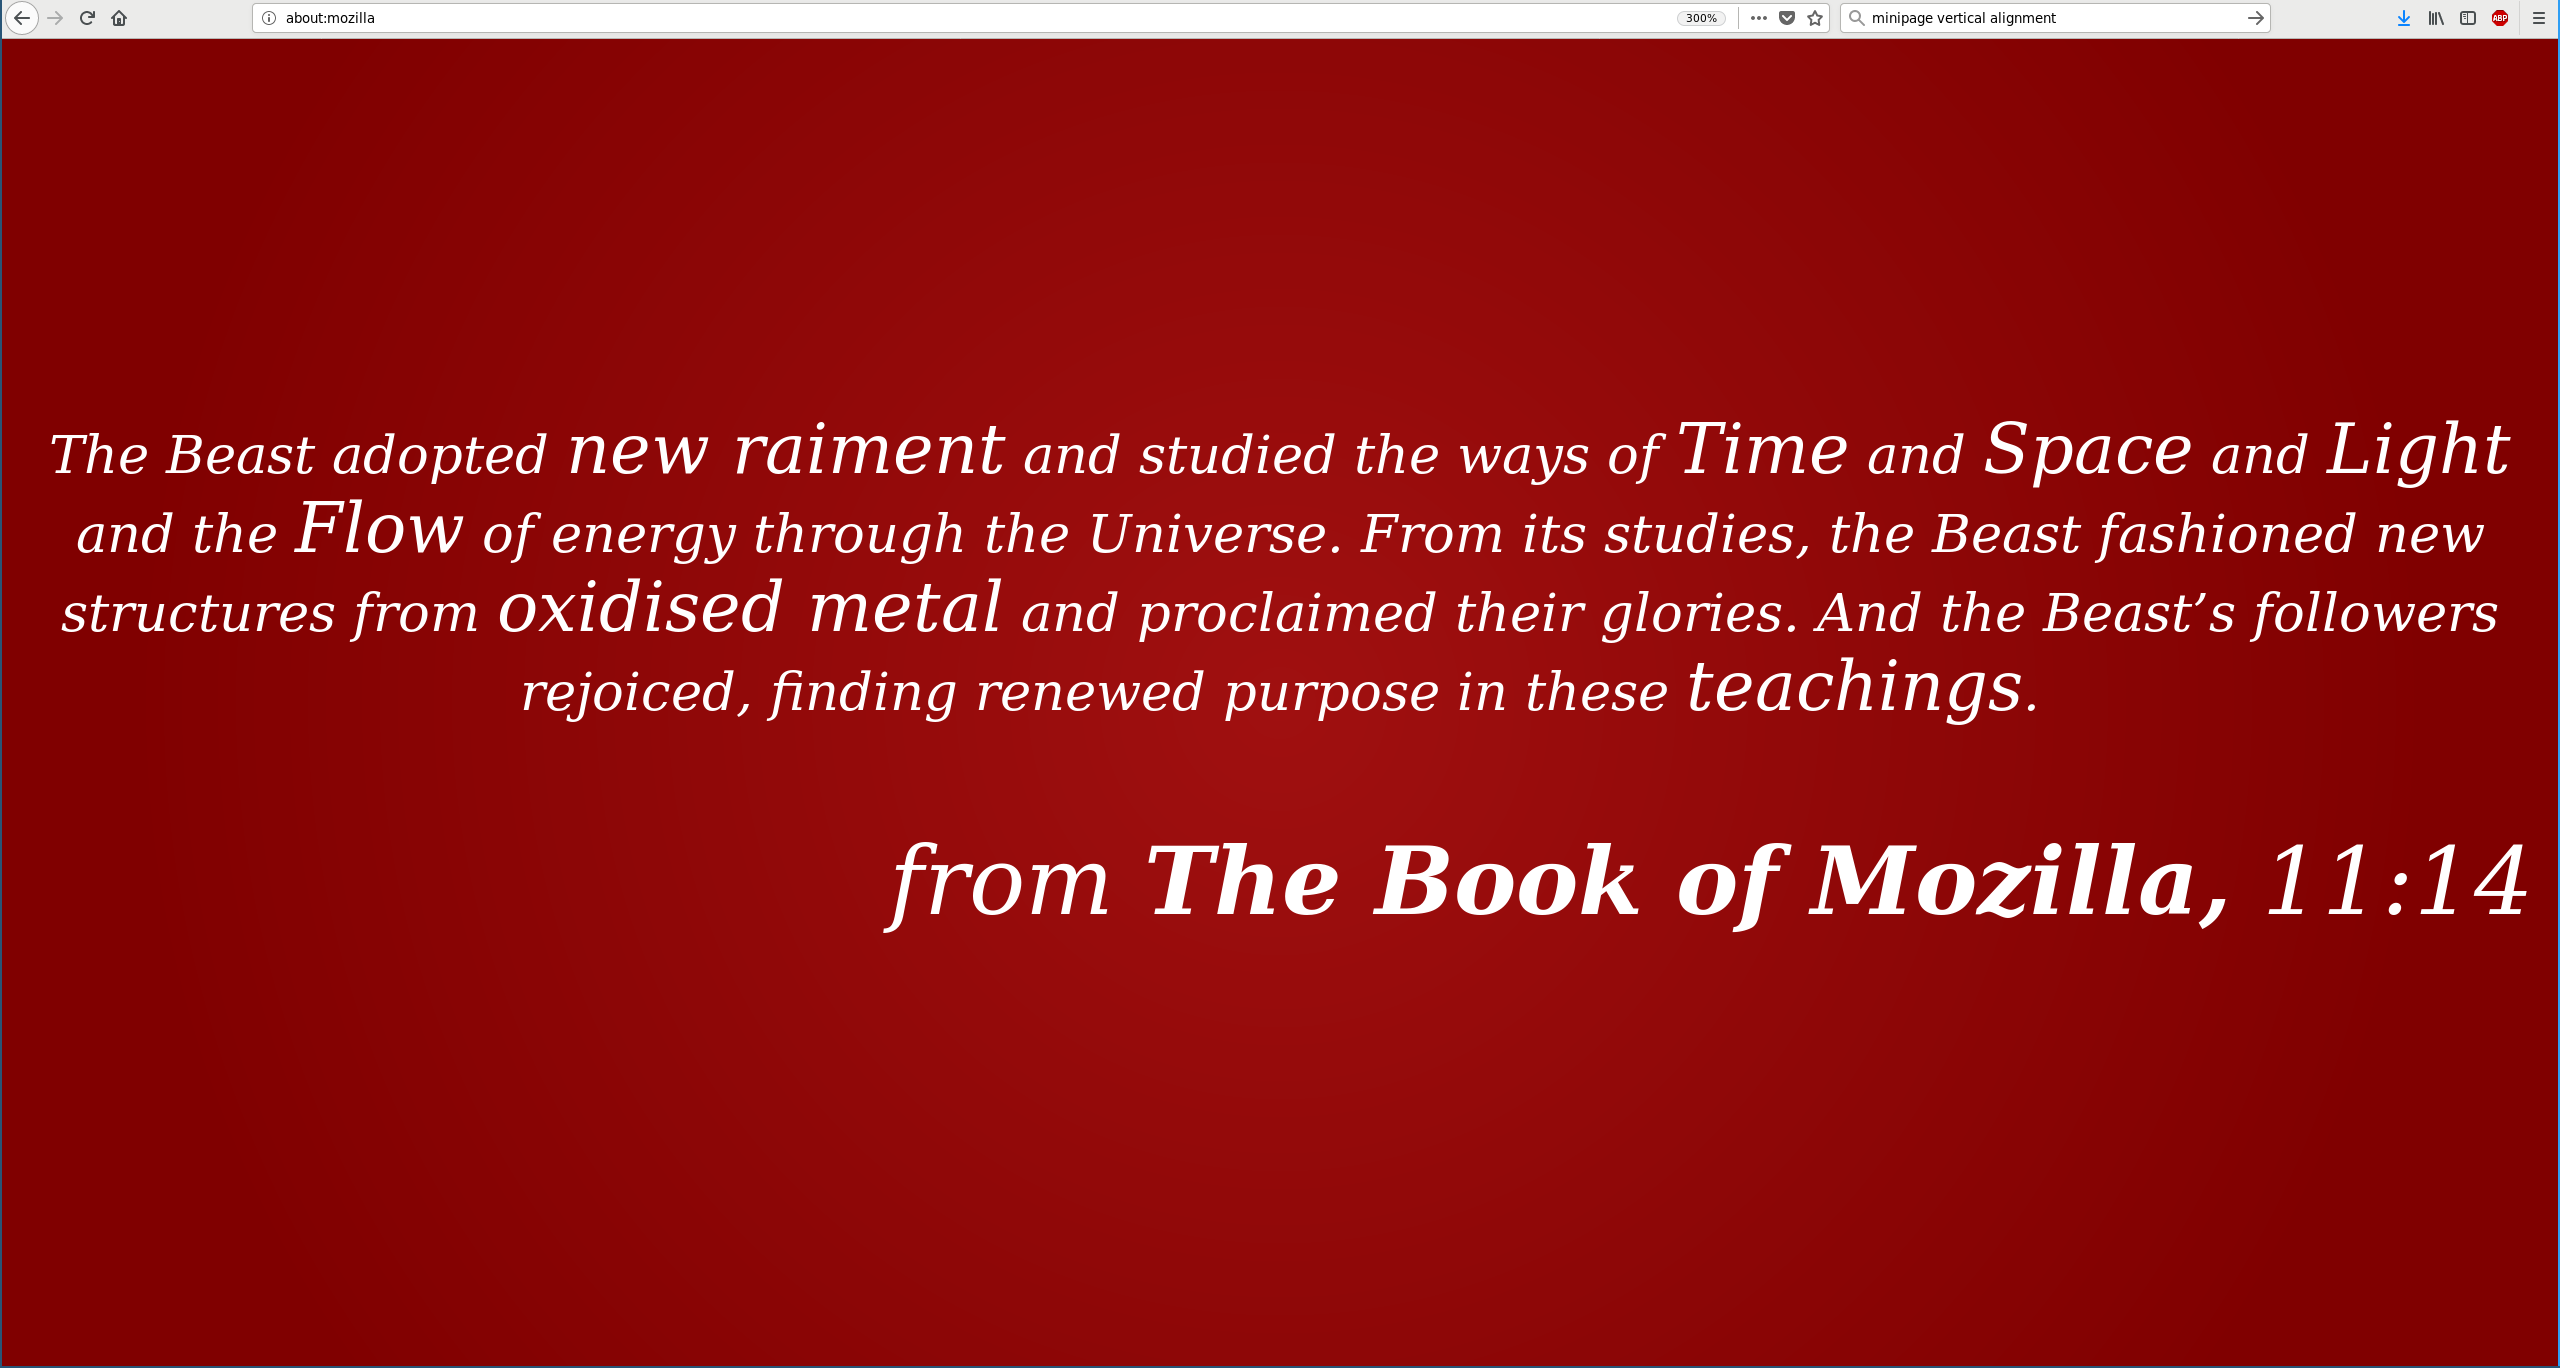
\includegraphics[width=\textwidth]{images/L19-about-mozilla.png}
\end{center}
\end{frame}

\begin{frame}
\frametitle{Faster Firefox Step 1: Electrolysis}

\Large
Electrolysis (2017): multiple OS-level processes.\\
(Think about threading models).

\begin{center}
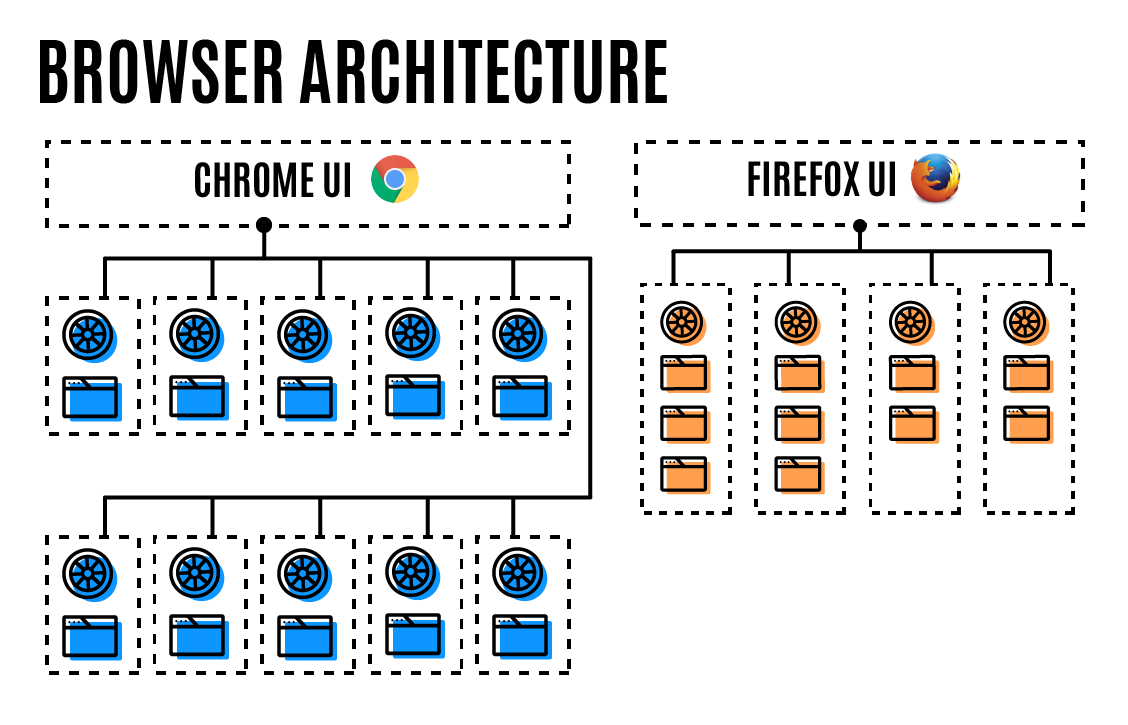
\includegraphics[width=.9\textwidth]{images/L19-chrome-vs-firefox.png}
\end{center}
\end{frame}

\begin{frame}
\frametitle{Chrome vs Firefox}

\Large
Chrome: 1-process-per-tab.\\
Firefox: 4 shared content processes.\\[1em]

Firefox uses less memory (has less render state).

Electrolysis challenges: \\
\qquad internal architecture, and add-ons.

\end{frame}

\begin{frame}
\frametitle{Electrolysis vs Flow}
\large
Two different Firefox projects:\\[1em]
\begin{changemargin}{2em}
Electrolysis = split across processes\\
\begin{tabbing}
Quantum Flow =~\=  leverage multithreading \\
\> (using Rust's ``fearless concurrency''), \\
\> plus other improvements.
\end{tabbing}
\end{changemargin}

\end{frame}

\begin{frame}
\frametitle{Quantum Flow}
\Large
\begin{changemargin}{1cm}
Steps:\\
\begin{enumerate}
\item Measure slowness \& prioritize
\item Gather help
\item Fix all (well, some of) the things!
\end{enumerate}

In 6 months:\\
\qquad prioritized 895 bugs, fixed 369.\\
Key tool: \\
\qquad ``Quantum Flow Engineering Newsletter''.
\end{changemargin}

\end{frame}

\begin{frame}
\frametitle{arewefastyet dot com}
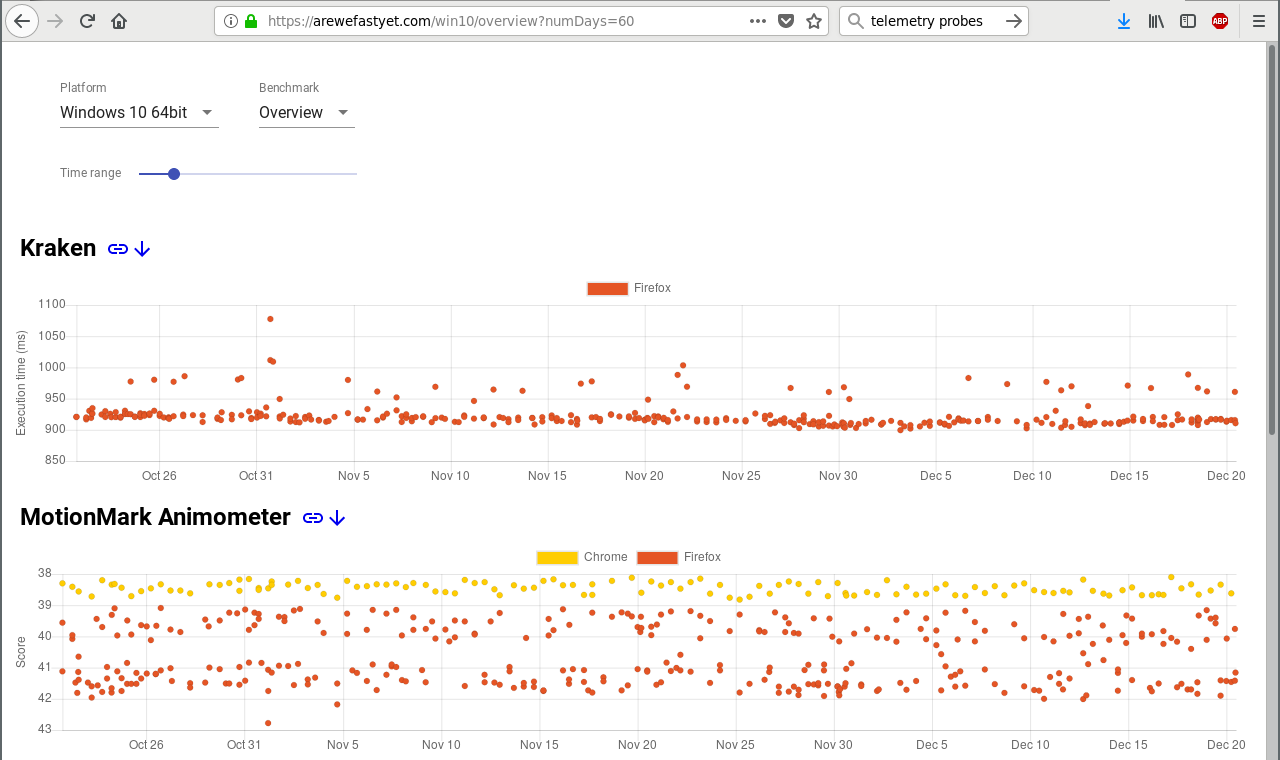
\includegraphics[width=.99\textwidth]{images/L19-arewefastyet.png}
\end{frame}

\begin{frame}
\frametitle{about:telemetry}
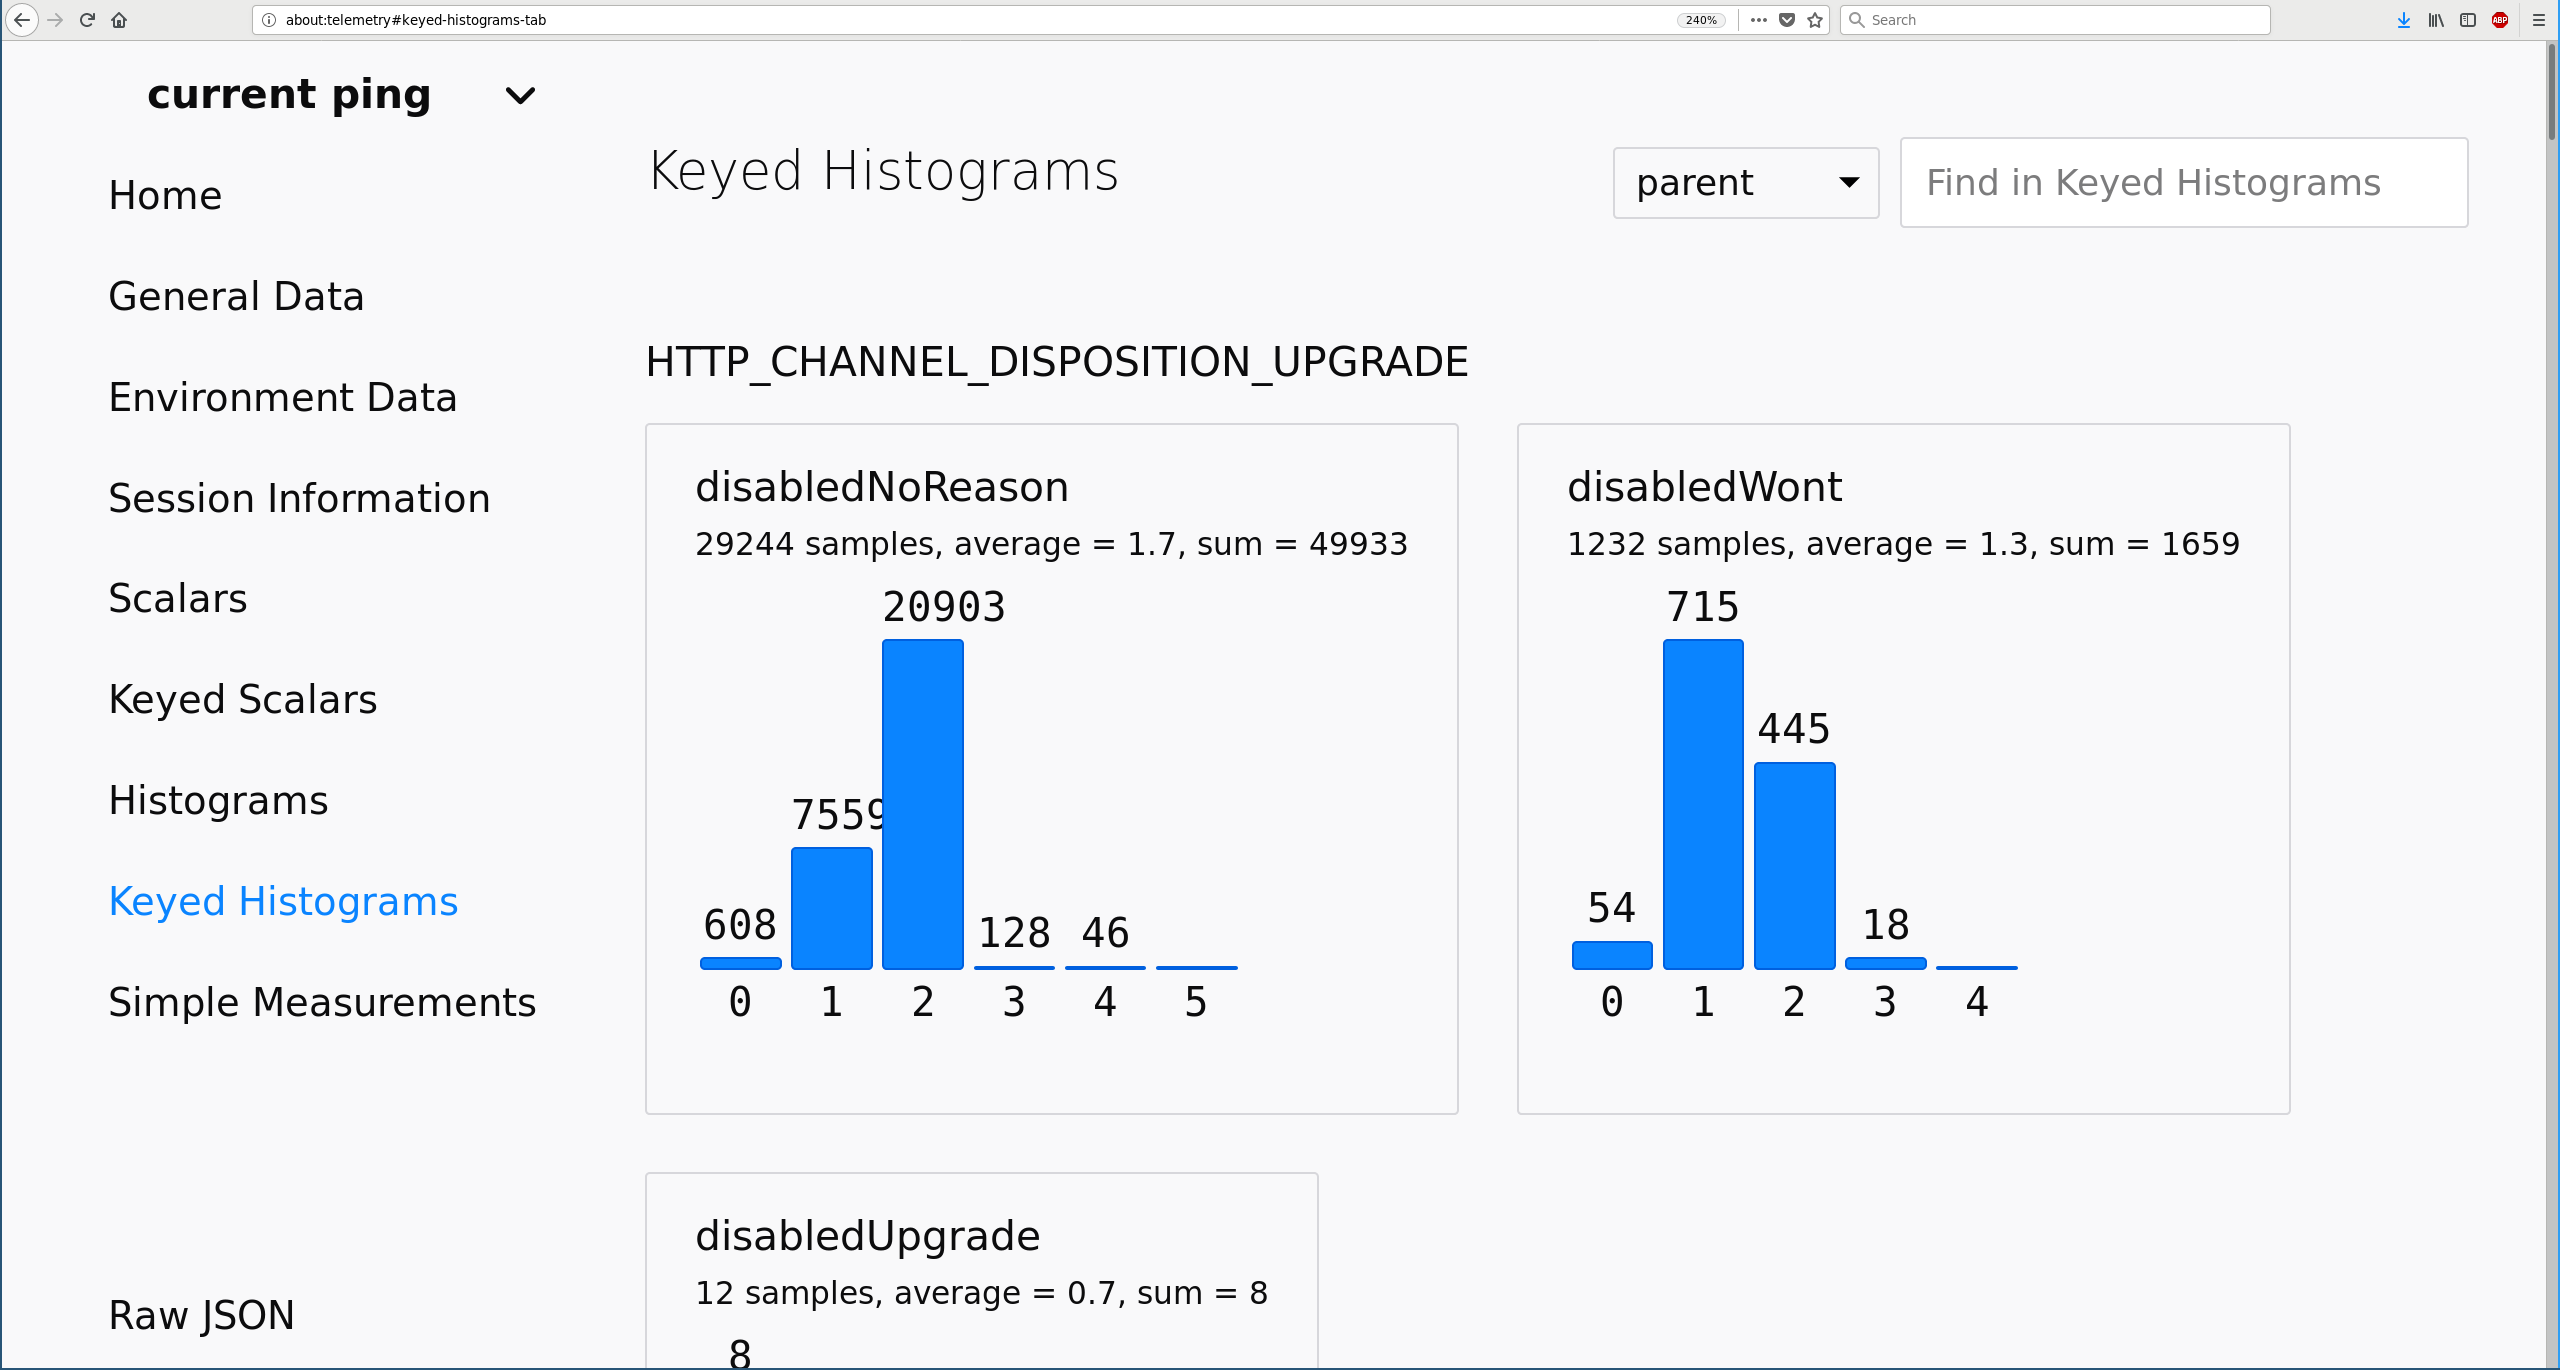
\includegraphics[width=.99\textwidth]{images/L19-about-telemetry.png}
\end{frame}

\begin{frame}
\frametitle{About Telemetry}
\Large
Idea: Ask questions first, act second.

Collect data about Firefox usage, then start hacking.

100s of GBs of anonymous metrics/day, \\
publicly available.

Analogous to CPU profiling, but massively distributed.
\begin{itemize}
\item collected much less often than CPU profiling data,\\
but at much broader scope.
\end{itemize}
\begin{center}
\url{https://telemetry.mozilla.org/}
\end{center}
\end{frame}

\begin{frame}
\frametitle{Example Telemetry Questions}
\Large
\begin{itemize}
\item Is Firefox the user's default browser? (69\% yes)
\item Does e10s make startup faster? (no, slower)
\item Which plugins tend to freeze the browser on load? (Silverlight and Flash)
\end{itemize}
Can also see evolution of data over time.
\end{frame}

\begin{frame}
\frametitle{ama}
\Large

Devs can propose new probes;\\
reviewed for data privacy plus normal code review.
\end{frame}

\begin{frame}
\frametitle{ping!}

\Large
Firefox sends pings:
\begin{itemize}
\item ``main ping'' every 24 hours;
\item upon shutdown;
\item upon environment change;
\item upon abnormal shutdown.
\end{itemize}
Presumably compressed JSON to Mozilla servers.

\end{frame}

\begin{frame}[fragile]
\frametitle{common ping structure}
\begin{verbatim}
{
  type: <string>, // "main", "activation", "optout", ...
  id: <UUID>, // a UUID that identifies this ping
  creationDate: <ISO date>, // the date the ping was generated
  version: <number>, // the version of the ping format

  application: {
    architecture: <string>, // build architecture, e.g. x86
    buildId: <string>, // "20141126041045"
    // etc
  },

  clientId: <UUID>, // optional
  environment: { ... }, // optional, not all pings contain
  payload: { ... }, // actual payload data for this ping type
}
\end{verbatim}
\end{frame}

\begin{frame}
\frametitle{Ping contents}
\Large

\begin{enumerate}
\item Scalars (counts, booleans, strings)
\item Histograms = bucketed data (like grade distributions)
\end{enumerate}

Both scalars and histograms can be keyed, \\
e.g. how often searches happen for which search engines.
\end{frame}

\part{Lower Level = Faster?}

\begin{frame}
\partpage
\end{frame}


\begin{frame}
\frametitle{OK Boomer}

\begin{center}
	
\includegraphics[width=0.5\textwidth]{images/grumpyman.jpg}
\end{center}


\end{frame}


\begin{frame}
  \frametitle{Introduction}

  
       C is low level, which is good for learning what's
    really going on.\\[2em]

    Writing compact, readable code in C is hard. \\ Common C sights:
      \begin{itemize}
        \item {\bf \#define macros}
        \item {\bf void*}
      \end{itemize}
    C++11 has made major strides towards readability and efficiency
      (it provides light-weight abstractions).
  
\end{frame}
%%%%%%%%%%%%%%%%%%%%%%%%%%%%%%%%%%%%%%%%%%%%%%%%%%%%%%%%%%%%%%%%%%%%%%%%%%%%%%%%

\section{Sorting}
%%%%%%%%%%%%%%%%%%%%%%%%%%%%%%%%%%%%%%%%%%%%%%%%%%%%%%%%%%%%%%%%%%%%%%%%%%%%%%%%
\begin{frame}[fragile]
  \frametitle{Goal}


  
  Sort a bunch of integers.\\[1em]
  In {\bf C}, usually use qsort from {\tt stdlib.h}.

  \begin{lstlisting}[language=C]
void qsort (void* base, size_t num, size_t size,
            int (*comparator) (const void*, const void*));
  \end{lstlisting}

  \begin{itemize}
    \item A fairly ugly definition (as usual, for generic C functions)
  \end{itemize}
  
\end{frame}
%%%%%%%%%%%%%%%%%%%%%%%%%%%%%%%%%%%%%%%%%%%%%%%%%%%%%%%%%%%%%%%%%%%%%%%%%%%%%%%%

%%%%%%%%%%%%%%%%%%%%%%%%%%%%%%%%%%%%%%%%%%%%%%%%%%%%%%%%%%%%%%%%%%%%%%%%%%%%%%%%
\begin{frame}[fragile]
  \frametitle{How ugly? {\tt qsort} usage}

  
  \begin{lstlisting}[language=C]
#include <stdlib.h>

int compare(const void* a, const void* b)
{
    return (*((int*)a) - *((int*)b));
}

int main(int argc, char* argv[])
{
    int array[] = {4, 3, 5, 2, 1};
    qsort(array, 5, sizeof(int), compare);
}
  \end{lstlisting}

  \begin{itemize}
    \item This looks like a nightmare, and is more likely to have bugs.
  \end{itemize}
  
\end{frame}
%%%%%%%%%%%%%%%%%%%%%%%%%%%%%%%%%%%%%%%%%%%%%%%%%%%%%%%%%%%%%%%%%%%%%%%%%%%%%%%%

%%%%%%%%%%%%%%%%%%%%%%%%%%%%%%%%%%%%%%%%%%%%%%%%%%%%%%%%%%%%%%%%%%%%%%%%%%%%%%%%
\begin{frame}[fragile]
  \frametitle{C++ {\tt sort}}

  
  C++ has a sort with a much nicer interface\footnote{\ldots nicer to use, after you get over templates (they're useful, I swear).}$\ldots$

  \begin{lstlisting}[language=C]
template <class RandomAccessIterator>
void sort (
    RandomAccessIterator first,
    RandomAccessIterator last
);

template <class RandomAccessIterator, class Compare>
void sort (
    RandomAccessIterator first,
    RandomAccessIterator last,
    Compare comp
);
  \end{lstlisting}
  
\end{frame}

%%%%%%%%%%%%%%%%%%%%%%%%%%%%%%%%%%%%%%%%%%%%%%%%%%%%%%%%%%%%%%%%%%%%%%%%%%%%%%%%

%%%%%%%%%%%%%%%%%%%%%%%%%%%%%%%%%%%%%%%%%%%%%%%%%%%%%%%%%%%%%%%%%%%%%%%%%%%%%%%%
\begin{frame}[fragile]
  \frametitle{C++ {\tt sort} Usage}

  
  \begin{lstlisting}[language=C]
#include <vector>
#include <algorithm>

int main(int argc, char* argv[])
{
    std::vector<int> v = {4, 3, 5, 2, 1};
    std::sort(v.begin(), v.end());
}
  \end{lstlisting}
  \vfill

  {\bf Note:} Your compare function can be a function or a functor. \\By~default,
  {\tt sort} uses {\tt operator$<$} on the objects being sorted.

  \begin{itemize}
    \item Which is less error prone?
    \item Which is {\bf faster}?
  \end{itemize}
  
\end{frame}
%%%%%%%%%%%%%%%%%%%%%%%%%%%%%%%%%%%%%%%%%%%%%%%%%%%%%%%%%%%%%%%%%%%%%%%%%%%%%%%%

%%%%%%%%%%%%%%%%%%%%%%%%%%%%%%%%%%%%%%%%%%%%%%%%%%%%%%%%%%%%%%%%%%%%%%%%%%%%%%%%
\begin{frame}
  \frametitle{Timing Various Sorts}


     The C++ version is {\bf twice} as fast. Why?
      \begin{itemize}
        \item The C version just operates on memory---it has no clue about the
          data.
        \item We're throwing away useful information about what's being sorted.
        \item A C function-pointer call prevents inlining of the compare function.
      \end{itemize}
     OK. What if we write our own sort in C, specialized for the data?
  
\end{frame}
%%%%%%%%%%%%%%%%%%%%%%%%%%%%%%%%%%%%%%%%%%%%%%%%%%%%%%%%%%%%%%%%%%%%%%%%%%%%%%%%

%%%%%%%%%%%%%%%%%%%%%%%%%%%%%%%%%%%%%%%%%%%%%%%%%%%%%%%%%%%%%%%%%%%%%%%%%%%%%%%%
\begin{frame}
  \frametitle{Custom Sort}


  \begin{itemize}
    \item The C++ version is still faster (although it's close).
    \item However, this is quickly going to become a maintainability nightmare.
      \begin{itemize}
        \item Would you rather read a custom sort or 1 line?
        \item What (who) do you trust more?
      \end{itemize}
  \end{itemize}
  

\end{frame}
%%%%%%%%%%%%%%%%%%%%%%%%%%%%%%%%%%%%%%%%%%%%%%%%%%%%%%%%%%%%%%%%%%%%%%%%%%%%%%%%

%%%%%%%%%%%%%%%%%%%%%%%%%%%%%%%%%%%%%%%%%%%%%%%%%%%%%%%%%%%%%%%%%%%%%%%%%%%%%%%%
\begin{frame}
  \frametitle{Lesson}
  
\large
    Abstractions don't always make your program slower. \\[1em]

    They 
      allow speedups and are much easier to maintain and read.
  
\end{frame}
%%%%%%%%%%%%%%%%%%%%%%%%%%%%%%%%%%%%%%%%%%%%%%%%%%%%%%%%%%%%%%%%%%%%%%%%%%%%%%%%

%%%%%%%%%%%%%%%%%%%%%%%%%%%%%%%%%%%%%%%%%%%%%%%%%%%%%%%%%%%%%%%%%%%%%%%%%%%%%%%%
\begin{frame}
  \frametitle{Lecture Fun}

  \begin{center}
\Large
    Let's throw Java-style programming (or at least collections) into the mix and see what happens.
    
    \begin{center}
	
\includegraphics[width=0.5\textwidth]{images/problemfactory.jpeg}
	\end{center}
    
  \end{center}
\end{frame}
%%%%%%%%%%%%%%%%%%%%%%%%%%%%%%%%%%%%%%%%%%%%%%%%%%%%%%%%%%%%%%%%%%%%%%%%%%%%%%%%

\section{Vectors vs. Lists}
%%%%%%%%%%%%%%%%%%%%%%%%%%%%%%%%%%%%%%%%%%%%%%%%%%%%%%%%%%%%%%%%%%%%%%%%%%%%%%%%
\begin{frame}
  \frametitle{Vectors vs. Lists: Problem}
  
  

    1. Generate {\bf N} random integers and insert them into (sorted)
      sequence.
      
  

      {\bf Example:} 3 4 2 1
      
      \begin{itemize}
        \item 3
        \item 3 4
        \item 2 3 4
        \item 1 2 3 4
      \end{itemize}
  

    2. Remove {\bf N} elements one at a time by going to a random position
      and removing the element.

  
      {\bf Example:} 2 0 1 0
      
      \begin{itemize}
        \item 1 2 4
        \item 2 4
        \item 2
        \item 
      \end{itemize}
  
  For which {\bf N} is it better to use a list than a vector (or array)?
  

\end{frame}
%%%%%%%%%%%%%%%%%%%%%%%%%%%%%%%%%%%%%%%%%%%%%%%%%%%%%%%%%%%%%%%%%%%%%%%%%%%%%%%%

%%%%%%%%%%%%%%%%%%%%%%%%%%%%%%%%%%%%%%%%%%%%%%%%%%%%%%%%%%%%%%%%%%%%%%%%%%%%%%%%
\begin{frame}
  \frametitle{Complexity}
  
  \begin{itemize}
    \item {\bf Vector}
      \begin{itemize}
        \item Inserting
          \begin{itemize}
            \item $O(\log n)$ for binary search
            \item $O(n)$ for insertion (on average, move half the elements)
          \end{itemize}
        \item Removing
          \begin{itemize}
            \item $O(1)$ for accessing
            \item $O(n)$ for deletion (on average, move half the elements)
          \end{itemize}
      \end{itemize}

    \item {\bf List}
      \begin{itemize}
        \item Inserting
          \begin{itemize}
            \item $O(n)$ for linear search
            \item $O(1)$ for insertion
          \end{itemize}
        \item Removing
          \begin{itemize}
            \item $O(n)$ for accessing
            \item $O(1)$ for deletion
          \end{itemize}
      \end{itemize}
  \end{itemize}
  \vfill
  Therefore, based on their complexity, lists should be better.
\end{frame}
%%%%%%%%%%%%%%%%%%%%%%%%%%%%%%%%%%%%%%%%%%%%%%%%%%%%%%%%%%%%%%%%%%%%%%%%%%%%%%%%

%%%%%%%%%%%%%%%%%%%%%%%%%%%%%%%%%%%%%%%%%%%%%%%%%%%%%%%%%%%%%%%%%%%%%%%%%%%%%%%%
\begin{frame}
  \frametitle{Reality}
 

  
  {\bf Vectors} dominate lists, performance wise. Why?
  \vfill
  \begin{itemize}
    \item Binary search vs. linear search complexity dominates.
    \vfill
    \item Lists use far more memory.

      {\bf On 64 bit machines:}
      \begin{itemize}
        \item Vector: 4 bytes per element.
        \item List: At least 20 bytes per element.
      \end{itemize}
    \vfill
    \item Memory access is slow, and results arrive in blocks:
      \begin{itemize}
        \item Lists' elements are all over memory, hence many
          cache misses.
        \item A cache miss for a vector will bring a lot more usable data.
      \end{itemize}
  \end{itemize}
  
\end{frame}
%%%%%%%%%%%%%%%%%%%%%%%%%%%%%%%%%%%%%%%%%%%%%%%%%%%%%%%%%%%%%%%%%%%%%%%%%%%%%%%%

%%%%%%%%%%%%%%%%%%%%%%%%%%%%%%%%%%%%%%%%%%%%%%%%%%%%%%%%%%%%%%%%%%%%%%%%%%%%%%%%
\begin{frame}
  \frametitle{Performance Tips: Bullets}

  
  \begin{itemize}
    \item Don't store unnecessary data in your program.
    \vfill
    \item Keep your data as compact as possible.
    \vfill
    \item Access memory in a predictable manner.
    \vfill
    \item Use vectors instead of lists by default.
    \vfill
    \item Programming abstractly can save a lot of time.
  \end{itemize}
  
\end{frame}
%%%%%%%%%%%%%%%%%%%%%%%%%%%%%%%%%%%%%%%%%%%%%%%%%%%%%%%%%%%%%%%%%%%%%%%%%%%%%%%%




\end{document}

